%%%%%%%%%%%%%%%%%%%%%%%%%%%%%%%%%%%%%%%%%%%%%%%%%%%%%%%%%%%%%%%%%%%%%%
% How to use writeLaTeX: 
%
% You edit the source code here on the left, and the preview on the
% right shows you the result within a few seconds.
%
% Bookmark this page and share the URL with your co-authors. They can
% edit at the same time!
%
% You can upload figures, bibliographies, custom classes and
% styles using the files menu.
%
%%%%%%%%%%%%%%%%%%%%%%%%%%%%%%%%%%%%%%%%%%%%%%%%%%%%%%%%%%%%%%%%%%%%%%



\documentclass[12pt]{article}

\usepackage{sbc-template} 
\usepackage{graphicx,url}

%\usepackage[brazil]{babel}   
\usepackage[utf8]{inputenc}  
\usepackage[document]{ragged2e}

     
\sloppy

\title{VPNs e seus usos na computação moderna\\ Artigo e Resumo}

\author{Pedro Henrique Bufulin de Almeida \inst{1}, Gabriel Solis Corrêa\inst{2},\\ Mateus Pereira da Silva\inst{3}, Bruno Falbo Zanotelli\inst{4} }

\address{Faculdade de Computação -- Universidade Federal de Uberlândia (UFU)
  \\Caixa Postal 593 -- CEP 38.400-902 -- Uberlândia -- MG -- Brazil
  \email{pedrohba18@gmail.com, gsolis.comp@gmail.com,}
  \email{mateus1128@gmail.com, brunofalbo@hotmail.com}
}

\begin{document}

\maketitle
     
\begin{resumo} 
  Presente Artigo visa explorar as VPNs, seus usos na computação moderna
  e ferramentas relacionadas, além de conceituar o termo VPN. Serão realizados
  e documentados testes utilizando a ferramenta OpenVPN em um sistema de máquinas Ubuntu,
  hospedados nos servidores da Digital Ocean, para observar o funcionamento e as
  limitações de uma VPN.
\end{resumo}


\section{O que é uma VPN?}

VPN, Virtual Private Network, ou melhor dizendo em português, Rede Virtual Privada,
vem se tornando cada vez mais comum no mercado tecnológico, encontramos nas lojas de aplicativos e softwares,
vários aplicativos de VPN, mas o que exatamente é uma VPN?
Resumidamente é um túnel seguro criado nada rede de comunicação entre o dispositivo e a Internet,
o que garante a segurança dos dados trafegados nessa rede de comunicação.
Em outra palavras, é codificar os dados que são trocados entre o dispositivo e a internet,
para tornar sua interceptação mais difícil, além de poder fornecer acesso restrito a quem tem as
credenciais necessárias. Extremamente recomendado para utilizar em locais com rede pública, como areoportos e shopping centers,
assim seus dados estariam criptografados, e se um invasor estiver analisando o trafego de dados,
encontrará apenas caracteres sem o menor sentido, porque seus dados de navegação estão todos criptografados,
evitando assim espionagem ("man-in-the-middle"), roubo de dados, ataque de hackers, entre outros.

\center
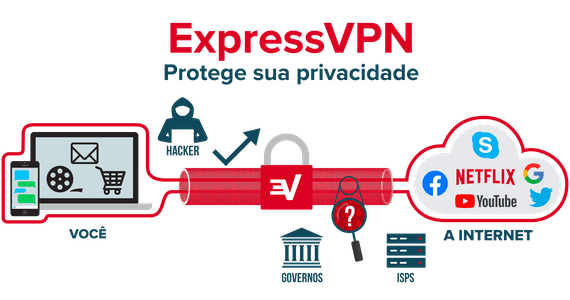
\includegraphics[width=10cm]{images/what-is-vpn-pt_3x.png}

\begin{flushleft}

\section{Definições e conceitos}

\subsection{Quais os protocolos são utilizados em VPN?}

Protocolos são essenciais na escolha do servidor VPN, já que é um elemento suma importância para esse serviço. 

Os protocolos são a combinação de padrões de criptografia e de transmissão, que concedem rápido acesso e segurança aos servidores VPN.

Existem vários tipos, dentre eles:


\subsubsection{PPTP}
Como uma extensão do Point-to-Point Protocol (PPP), o PPTP (Point-to-Point Tunneling Protocol) é um protocolo de servidor VPN muito utilizado e suportado pelos dispositivos. Ele possui uma criptografia mais básica, o que pode deixar a desejar na questão de segurança dos dados. 

Contudo, essa característica também faz com que ele seja mais rápido do que outros modelos de protocolo VPN, além de possuir configuração mais simples. A maior parte das falhas de segurança também já foram resolvidas nas versões mais atuais do PPTP. Isso faz com que essa maior agilidade compense em detrimento de uma menor segurança para algumas empresas.

Uma forma de melhorar a segurança é utilizar da tecnologia PPP ou Protocolo Ponto-a-Ponto para implementar medidas de criptografia.

Esta é uma VPN útil tanto para os usuários empresariais, como, para usuários domésticos. São ideais para uso pessoal e empresarial, porque elas não exigem a compra e a instalação de hardware e recursos extras, normalmente oferecidos como software add-on barato. Além de serem compatíveis com os sistemas Linux, Windows e Mac.

\subsubsection{L2TP}
O L2TP (Layer 2 Tunneling Protocol) consegue garantir confidencialidade, autenticação e integridade de dados, o que assegura maior proteção. No entanto, nada disso é oferecido pelo protocolo por si só. Pois ele se baseia em um protocolo de criptografia IPSec para proporcionar a privacidade necessária aos usuários da rede.

As ligações do L2TP são conhecidas como linhas virtuais e oferecem mais facilidades para aqueles que utilizam o servidor de forma remota. Isso porque ele possibilita que o servidor da rede VPN de uma organização consiga gerir os endereços IP atribuídos aos seus usuários. Assim, garantindo proteção e privacidade.

\subsubsection{IPSec}
IPSec (Internet Protocol Security) oferece transferência estável de dados pela rede pública ou privada. Uma extensão do protocolo IP (Internet Protocol), ele visa garantir mais segurança na comunicação, utilizando-se de serviços de segurança criptográficos. 

Sua forma de funcionamento se dá da seguinte maneira: é necessário pegar um pacote IP privado, criptografar, autenticar e dar integridade e depois encapsular os pacotes protegidos para novos IPs a serem repassados.

Com esta maneira operacional, o IPSec se torna um bom protocolo em segurança para as empresas, filiais e usuários remotos. Dentre as suas principais vantagens e benefícios, podemos destacar também o oferecimento de um alto nível de confidencialidade, privacidade e autenticação dos dados e informações que trafegam dentro da rede.


\subsection{Pontos fortes e fracos de uma VPN}

O uso de um servidor VPN é principalmente recomendado para empresas. Pois consegue manter informações seguras nas comunicações remotas ou em armazenamento em nuvem.

Servidores com tal configuração, trazem algumas vantagens para os usuários, como:

\subsubsection{Segurança}

Principal ponto positivo do servidor VPN.  Por usar criptografia dos dados e diversos outros recursos de segurança, ele permite que a navegação seja mais confiável e segura, independente de onde seja usada e em qual rede acessada.

\subsubsection{Privacidade}
As informações que estão na rede só são acessadas por quem tem permissão. Assim, cada indivíduo tem acesso apenas ao que é de seu interesse para o trabalho e nada mais. Dessa forma, todas as informações e dados que circulam dentro da rede da empresa acabam sendo mais confiáveis e úteis. 

A privacidade dos usuários que utilizam a rede com servidor VPN estará garantida, sem riscos de que informações confidenciais sejam vazadas.

\subsubsection{Acesso remoto}
Desde que, aqueles com permissão tenham acesso a internet, será garantido acessar os servidores remotos, não importando o lugar do mundo ou o dispositivo. 

Tal característica permite que, funcionários trabalhem remotamente sem que precisem carregar notebooks da empresa ou anotem informações importantes quando tiverem a distância. Tornando o trabalho mais simples e tendo um ganho considerável em produtividade.

A empresa também se beneficia pois, deixa de ser necessário investir em equipamentos e tecnologias que garantiriam o acesso e segurança aos sistemas. Assim como funcionários podem passar a usar seus próprios dispositivos.

\subsubsection{Custo}
Servidores VPN são consideravelmente mais baratos do que outras tecnologias e configurações de segurança.

Como utilizam a rede pública de internet como conexão, diminui-se os custos de implantação e softwares próprios.


Porém, todo e qualquer sistema ou tecnologia apresentam desvantagens, no caso de servidores VPN, essas são as principais:

\subsubsection{Velocidade}
Principal ponto negativo de servidores VPN. Para utilizar esse tipo de servidor é preciso estabelecer duas conexões.

Logo, uma boa velocidade de rede é exigida, e mesmo assim, é quase sempre bem perceptível a queda na banda de internet utilizada.

\subsubsection{Dependência da Internet}
O acesso remoto é algo extremamente útil para se trabalhar fora da empresa porém, um acesso constante a internet é necessário.

Se a rede tem uma conexão instável, cai frequentemente ou se não possui acesso a internet, não será possível acessar o servidor VPN e os dados nele armazenados.

\subsubsection{Confiança no Servidor}
Existem muitos serviços de VPN sendo oferecidos, alguns gratuitos, a preços baixos ou outros que necessitam de um investimento maior.

Com tanta oferta, é importante entender as necessidades da sua rede, antes de contratar algum serviço.  As VPNs constantemente mudam. Por isso, é importante ter um suporte em que a empresa consiga facilmente entrar em contato para resolver os impasses da rede.

Uma outra opção, seria a empresa criar a sua própria rede de servidores VPN, utilizando tecnologias Open Source, tais como, a OpenVPN. Tópico esse, que será abordado mais a frente.


\subsubsection{VPN vs SSL}

Uma rápida pesquisa sobre criptografia e segurança de dados é o suficiente para encontrar as duas siglas. E por vezes, é possível confundir o funcionamento de uma com a outra. Porém, ambas tecnologias, apesar de visar segurança (simplificando), não são a mesma e operam de formas diferentes.

VPN e SSL não são do mesmo nível. Uma implementação de VPN requer alguma criptografia em algum ponto. Algumas implementações inclusive, usam SSL, resultando em um sistema em camadas.

Nesse caso, o servidor  VPN transfere pacotes IP em uma conexão SSL, que por sua vez usa TCP como meio de transporte. O IPsec é outra tecnologia que está mais profundamente integrada nos pacotes, o que suprime algumas dessas camadas e, portanto, é um pouco mais eficiente (menos sobrecarga de largura de banda). 

Por outro lado, o IPsec deve ser gerenciado profundamente no código de rede do sistema operacional, enquanto uma VPN baseada em SSL só precisa de alguma forma de sequestrar o tráfego de entrada e saída. O resto pode estar no software de nível de usuário.

A principal diferença é que o SSL costuma fazer uso do navegador para criptografar dados entre o usuário final e o servidor, sendo comumente utilizado para áreas de sites que exigem a proteção da confidencialidade e integridade dos dados. VPN / IPSEC requer software VPN Client específico e geralmente é para fornecer acesso remoto a sistemas ou redes.

No entanto, as VPNs SSL estão se tornando mais predominantes como meio de fornecer acesso a redes / sistemas por meio do navegador da web. Essa abordagem tem muitos benefícios, pois usa o navegador da web comum para habilitar a conexão segura. A granularidade dessa abordagem também é uma boa maneira de controlar o acesso a aplicativos específicos.


\section{Configurado uma VPN utilizando OpenVPN}


\subsection{Requisitos}

Para que seja possível implementar uma VPN como neste exemplo, você precisará
de uma máquina rodando Ubuntu versão 18.04. Por questões de praticidade, não será
visto com profundidade todo o processo de instalação das ferramentas que serão usadas, sendo algumas 
apenas mencionadas cabendo ao leitor descobrir como instalá-las. Além do servidor mencionado,
o ideal seria ter uma outra máquina para ser a autoridade de certificação (CA), para evitar
que um agressor capaz de se infiltrar no servidor consiga acessar a chave privada
e assinar novos certificados. 

\subsection{Instalando os programas necessários}

O primeiro passo é instalar o \emph{OpenVPN} que está disponível nos repositórios padrão do ubuntu.
Em seguida, instale \emph{EasyRCA} tanto na máquina CA quanto no servidor que servira o VPN.
O repositório deste programa encontra-se no github no mesmo repositório do \emph{OpenVPN}. 
A versão a ser utilizada é a 3.0.8.

\subsection{Configurando as variáveis e construindo o CA}

No máquina que contém o CA, entre no diretório onde foi extraído o \emph{EasyRCA}. copie o conteúdo
do arquivo \texttt{vars.example} para um outro arquivo onde serão armazenadas as variáveis. Atualize
os valores de acordo com suas informações, feche e salve o arquivo. 

Dentro do da mesma pasta, existe um\emph{script} chamado \texttt{easyrca}. Execute-o da seguinte
maneira: \texttt{./easyrsa init-pki}. Isso irá iniciar a infraestrutura de chaves públicas no servidor CA.
Se der tudo certo, deve surgir um diretório chamado \texttt{pki}. Em seguida, chame o script anterior 
novamente mas dessa vez com a opção \texttt{build-ca}. Isso irá construir a CA e criar
dois arquivos importantes. Um deles é um certificado público que no contexto de uma VPN para informar
ao servidor e ao cliente que ambos fazem parte da mesma rede. Isso serve como defesa de ataques 
do tipo \emph{man-in-the-middle} 
-

\section{Discussão}

Esse artigo discorreu sobre o conceito e a usabilidade das VPNs, de modo a observar também a importância
do seu uso no contexto da internet contemporânea. Além disso, o artigo buscou analisar a implementação
dessas ferramentas e também uma forma de hospedar a sua própria VPN.

Desse modo, levanta-se também uma discussão sobre como os diferentes usos das VPNs se aplicam no cotidiano.
Assim, é necessário questionar, por exemplo, qual a abordagem da VPN uma pessoa leiga à
computação, mas que frequentemente faz uso de computadores no seu cotidiano, deveria utilizar.
Mesmo com as ferramentas atuais, observa-se que, para um iniciante na àrea, configurar e hospedar
uma VPN própria pode ser difícil ou pouco intuitivo.
Por consequência, a solução que este usuário pode recorrer é utilizar algum serviço de VPN disponível
na internet e confiar que seja seguro. 
Com isso, uma segunda problemática é colocada em pauta, já que ao escolher um serviço de VPN, 
surge o questionamento de qual seria o modelo mais adequado e seguro para o usuário, isto é, se é melhor
contratar um serviço pago ou optar por um serviço gratuito de VPN.
No quesito segurança e confiabilidade, os serviços pagos sem dúvida são os adequados quando essas
são as principais preocupações do usuário.
Já o serviço gratuito tem a variável preço como principal fator de adesão, mas por outro lado, existem
grandes chances da segurança ser comprometida, já que é possível que o provedor faça uso ou até venda
as suas informaçoês para terceiros para pagar os custos do serviço dele.
Dessa forma, o serviço pago é o mais adequado para esses usuários que optam por utilizar um serviço de
terceiros em vez de configurar sua VPN por conta própria. 


\section{Considerações Finais}

É desnecessário dizer que, é fundamental cuidar da segurança e proteção das informações da sua empresa, ou de seus dados pessoais e a VPN é uma das ferramentas essenciais nesse cuidado.

Para o primeiro cenário, VPN é um mecanismo muito importante dentro do ambiente empresarial, e fazer o acesso remoto sem utilizá-la é colocar os dados e informações da sua empresa em risco.

Além disso, tal tecnologia, pode trazer uma série de benefícios para a empresa como: Segurança nos dados, corte de gastos, aumento de produtividade, entre outros.

Já no uso doméstico a VPN se torna uma ferramenta tão importante quanto. 

Independente de estar num ambiente totalmente livre e aberto ou em um com alto nível de monitoramento, usar uma VPN garante que suas comunicações se tornem seguras e criptografadas, longe de olhos de curiosos e pessoas má intencionadas.

Também é possível ganhar acesso a conteúdos e informações que estariam bloqueados para seu país ou região. Assim como garantir a liberdade de expressão, pelo anonimato, em locais que essa “prática” não é assegurada. 

Em suma, servidores VPN são uma poderosa ferramenta na busca por privacidade e segurança de informação. O seu funcionamento pode parecer complexo, e sua implementação complicada, no caso de uma rede própria, mas no final para quem busca esses pontos, a VPN se torna sua maior aliada.



\bibliographystyle{sbc}
\bibliography{sbc-template}

\cite{hostone:100}
\cite{stackexchange:101}
\cite{compugraf:103}
\cite{starti:104}

\end{flushleft}
\end{document}
